
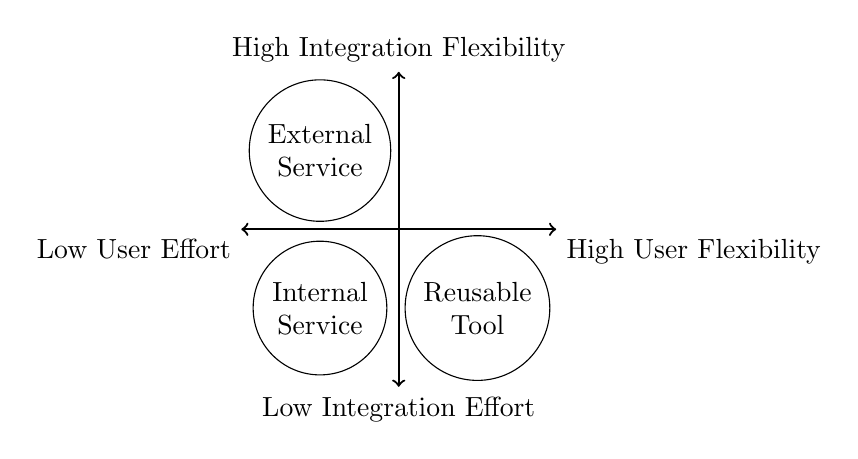
\begin{tikzpicture}[scale=1, every node/.style={scale=1}]

    % Draw axes
    \draw[thick,->] (0,0) -- (2,0) node[anchor=north west] {High User Flexibility};
    \draw[thick,->] (0,0) -- (0,2) node[anchor=south ] {High Integration Flexibility};
    \draw[thick,->] (0,0) -- (-2,0) node[anchor=north east] {Low User Effort};
    \draw[thick,->] (0,0) -- (0,-2) node[anchor=north ] {Low Integration Effort};

    % Add the three combinations
    % Reusable Service: Low Integration Effort and Low User Effort
    \node[align=center, draw, circle] (RS) at (-1,-1) {Internal\\Service};

    % Platform Tool: Low Integration Effort and High User Flexibility
    \node[align=center, draw, circle] (PT) at (1,-1) {Reusable\\Tool};

    % Platform Service: Low User Effort and High Integration Flexibility
    \node[align=center, draw, circle] (PS) at (-1,1) {External\\Service};

\end{tikzpicture}

